\documentclass[fleqn]{article}
\usepackage{amsmath}
\usepackage[dvips]{graphicx}
\bibliographystyle{plain}
%__________________________________SHOCKTUBE 1 level
\begin{document}

\section*{\center Shock Tube}
\subsection*{\underline{Problem Description}}
The shock tube problem is a standard 1D compressible flow problem that has been used by many as a
validation test case \cite{laney, sod, toro}.  At time $t=0$ the computational domain is divided
into two separate regions of space by a diaphram, with each region at a different density and
pressure.  The separated regions are at rest with a uniform temperature $=300K$.  The initial
pressure ratio is $\frac{P_R}{P_L}  = 10$ and density ratio is $\frac{\rho_R}{\rho_L} = 0.1$  The
diaphram is instantly removed and a traveling shockwave, discontinutity and expansion fan form.  The
expansion fan moves towards the left while the shockwave and contact discontinutity move to the
right.  This problem tests the algorithm's ability to capture steep gradients and solve Eulers equations. 
 
\subsection*{\underline{Simulation Specifics}}
\begin{description} 
\item [Component used:] \hfill ICE
\item [Input file name:] \hfill shocktube.ups
\item [Command used to run input file:]\hfill sus shocktube.ups
\item [Postprocessing command:]\hfill \\
inputs/UintahRelease/ICE/plot\_shockTube\_1L shockTube.uda

\item [Simulation Domain:]\hfill    1 x .01 x .01 m
\item [Cell Spacing:]\hfill \\ 
0.1 x 10 x 10 mm (Level 0)

\item [Example Runtimes:] \hfill \\
 2 minutes   (1 processor, 2.4 GHz Xeon)

\item [Physical time simulated:] \hfill 0.005 sec.

\end{description}

\section*{\underline{Results}}
Figure \ref{results.ST} shows a comparison of the exact versus simulated results at time $t = 5msec$.
\begin{figure}
\includegraphics[scale=.85]{figures/shockTube.ps}
\caption{Shock tube results at time $t = 5msec$}
\label{results.ST}
\end{figure}
\newpage

%__________________________________SHOCKTUBE AMR

\section*{\center Shock Tube with AMR}
 
\subsection*{\underline{Simulation Specifics}}
\begin{description} 
\item [Component used:] \hfill ICE
\item [Input file name:] \hfill shocktube\_AMR.ups
\item [Command used to run input file:]\hfill sus shocktube\_AMR.ups
\item [Postprocessing command:]\hfill \\
inputs/UintahRelease/ICE/plot\_shockTube\_AMR shockTube\_AMR.uda

\item [Simulation Domain:]\hfill    1 x .01 x .01 m
\item [Cell Spacing:]\hfill \\ 
0.1 x 10 x 10 mm (Level 0)
0.025 x 10 x10 mm (Level 1)
0.00625 x10 x10 mm (Level 2)


\item [Example Runtimes:] \hfill \\
 2ish minutes   (1 processor, 2.4 GHz Xeon)

\item [Physical time simulated:] \hfill 0.005 sec.

\end{description}

\section*{\underline{Results}}
Figure \ref{results.ST.AMR} shows a comparison of the exact versus simulated results at time $t = 5msec$.
\begin{figure}
\includegraphics[scale=.85]{figures/shockTube_AMR.ps}
\caption{Shock tube results at time $t = 5msec$}
\label{results.ST.AMR}
\end{figure}
\newpage

%__________________________________Single level blast wave

\section*{\center BlastWave 2D}
\subsection*{\underline{Problem Description}}
The Sedov-Taylor blastwave problem is a standard compressible flow problem that has been used by many
as a validation test case.  At time $t=0$ there is a small region of gas at the center of the domain
at a relatively high temperature and pressure.  The expansion of high pressure gas forms a spherical
blast wave that expands into surrounding atmosphere.
\subsection*{\underline{Simulation Specifics}}
\begin{description} 
\item [Component used:] \hfill ICE
\item [Input file name:] \hfill blastWave.ups
\item [Command used to run input file:]\hfill sus blastWave.ups
\item [Visualization net file:]\hfill blastWave\_1L.srn\\


\item [Simulation Domain:]\hfill    1 x 1 x .05 m
\item [Cell Spacing:]\hfill \\ 
5 x 5 x 50 mm (Level 0)


\item [Example Runtimes:] \hfill \\
 9ish minutes   (1 processor, 2.4 GHz Xeon)

\item [Physical time simulated:] \hfill 0.9e-3sec.

\end{description}

\section*{\underline{Results}}
Figure \ref{results.BW} shows a comparison of the exact versus simulated results at time $t = 5msec$.
\begin{figure}
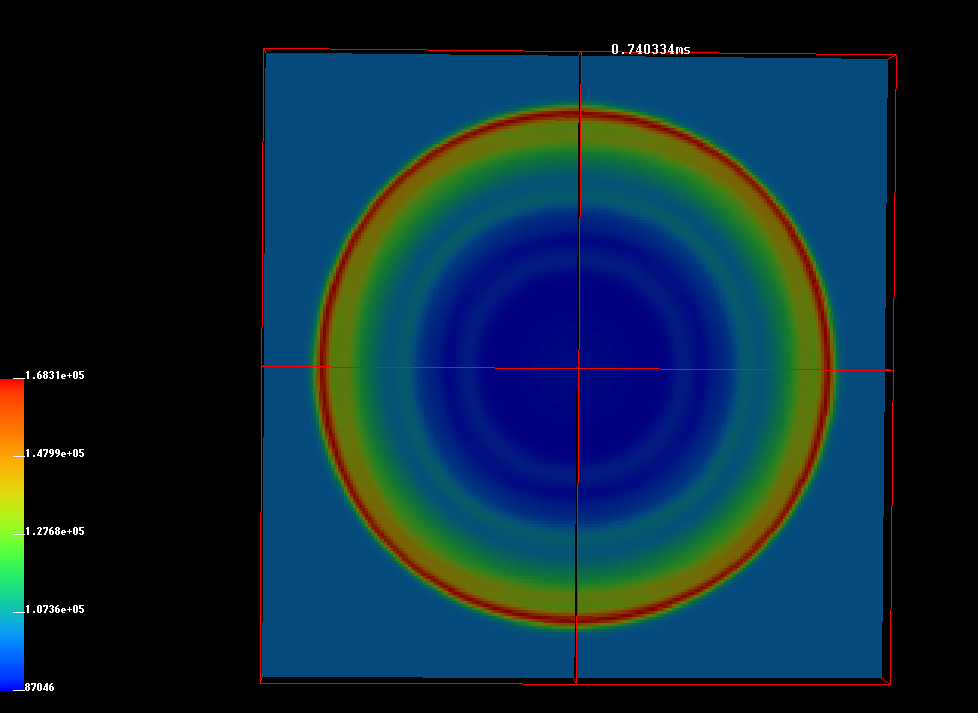
\includegraphics[scale=.5]{figures/blastWave.ps}
\caption{Pressure field at time $t = 0.74msec$}
\label{results.BW}
\end{figure}
\newpage

%__________________________________AMR blast wave

\section*{\center BlastWave AMR}
\subsection*{\underline{Simulation Specifics}}
\begin{description} 
\item [Component used:] \hfill ICE
\item [Input file name:] \hfill blastWave.ups
\item [Command used to run input file:]\hfill sus blastWave\_AMR.ups
\item [Visualization net file:]\hfill blastWave\_1L.srn\\


\item [Simulation Domain:]\hfill    1 x 1 x .05 m
\item [Cell Spacing:]\hfill \\ 
20 x 20 x 50 mm (Level 0) 
5 x 5 x 50 mm (Level 1)


\item [Example Runtimes:] \hfill \\
 9ish minutes   (1 processor, 2.4 GHz Xeon)

\item [Physical time simulated:] \hfill 0.9e-3sec.

\end{description}

\section*{\underline{Results}}
Figure \ref{results.BW.AMR} shows the pressure field and an outline of the individual patches on
levels 0 \& 1.  This simulation shows the adaptive mesh capabilities of ICE and the UCF.  
\begin{figure}
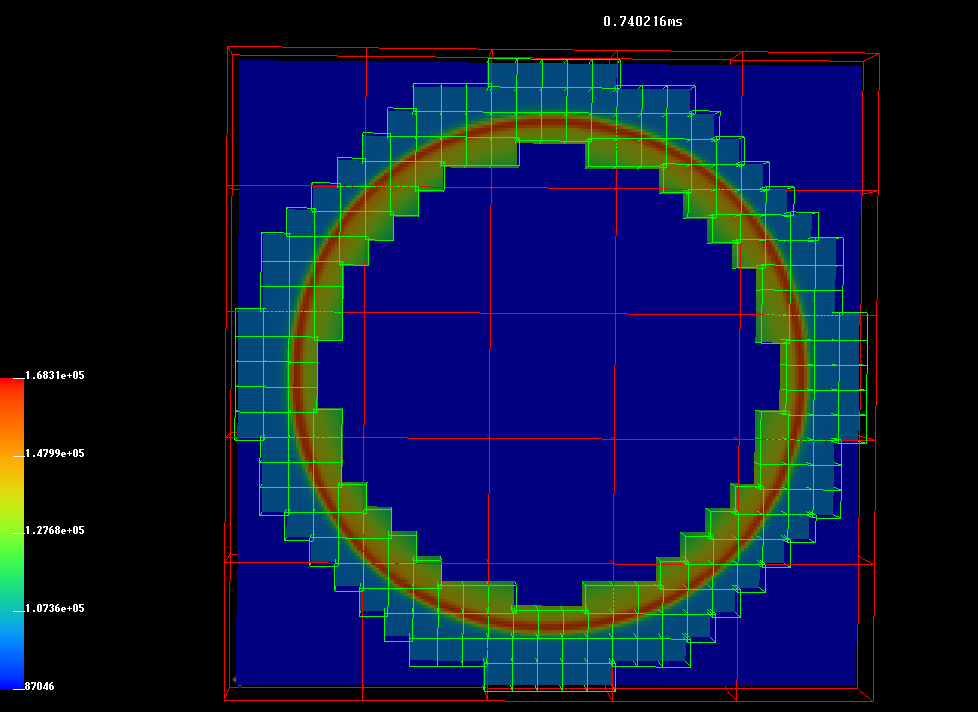
\includegraphics[scale=.5]{figures/blastWave_AMR.ps}
\caption{Pressure field at time $t = 0.74msec$.  The individual patches on levels 0 \& 1 are shown.}
\label{results.BW.AMR}
\end{figure}
Good agreement between the single level results (Fig. \ref{results.BW}) and the AMR results (Fig.
\ref{results.BW.AMR}) is shown.
\newpage

%__________________________________CH4 fire

\section*{\center Methane Flame}
\subsection*{\underline{Problem Description}}
At $t=0$ Methane gas begin flowing from a $1m$ hole in the floor of the computational domain at a
velocity of $1m/s$.  The methane mixes with the surrounding air, ignites and forms a puffing fire. 
The main assumptions in this simulation are a) that the chemical reactions are taking place infinitely
fast (equilibrium chemistry model) and b) that there is no radiative heat loss from the product
gases.
\subsection*{\underline{Simulation Specifics}}
\begin{description} 
\item [Component used:] \hfill ICE
\item [Input file name:] \hfill CH4\_fire.ups
\item [Command used to run input file:]\hfill sus CH4\_fire.ups \\
Note you must have a link to the {\tt inputs} directory in the save directory as sus.  A table needed
by the combustion model is inside the {\tt inputs} directory.
\item [SCIRun visualization net file:]\hfill 3DFire\_Vol.srn \\


\item [Simulation Domain:]\hfill    5 x 5 x 5 m
\item [Cell Spacing:]\hfill \\ 
3.3 x 3.3 x 3.3 cm (Level 0)


\item [Example Runtimes:] \hfill \\
 8 hours   (64 processor, 2.4 GHz Xeon)

\item [Physical time simulated:] \hfill 3.4sec.

\end{description}

\section*{\underline{Results}}
Figure \ref{results.CH4} shows a 3D view of the initial puff just before it leaves the computational
doman.  
\begin{figure}
\includegraphics[scale=.66]{figures/3DFire.ps}
\caption{Temperature field at time $t = 1.5 sec$}
\label{results.CH4}
\end{figure}
\newpage


\bibliography{../references}

\end{document}
